%%=============================================================================
%% Methodologie
%%=============================================================================

\chapter{\IfLanguageName{dutch}{Methodologie}{Methodology}}%
\label{ch:methodologie}

%% TODO: In dit hoofstuk geef je een korte toelichting over hoe je te werk bent
%% gegaan. Verdeel je onderzoek in grote fasen, en licht in elke fase toe wat
%% de doelstelling was, welke deliverables daar uit gekomen zijn, en welke
%% onderzoeksmethoden je daarbij toegepast hebt. Verantwoord waarom je
%% op deze manier te werk gegaan bent.
%% 
%% Voorbeelden van zulke fasen zijn: literatuurstudie, opstellen van een
%% requirements-analyse, opstellen long-list (bij vergelijkende studie),
%% selectie van geschikte tools (bij vergelijkende studie, "short-list"),
%% opzetten testopstelling/PoC, uitvoeren testen en verzamelen
%% van resultaten, analyse van resultaten, ...
%%
%% !!!!! LET OP !!!!!
%%
%% Het is uitdrukkelijk NIET de bedoeling dat je het grootste deel van de corpus
%% van je bachelorproef in dit hoofstuk verwerkt! Dit hoofdstuk is eerder een
%% kort overzicht van je plan van aanpak.
%%
%% Maak voor elke fase (behalve het literatuuronderzoek) een NIEUW HOOFDSTUK aan
%% en geef het een gepaste titel.

Volgende hoofdstukken verlopen in sequentiële volgorde om dit onderzoek in de juiste richting te sturen.
De literatuurstudie geeft een basis om verdere vakterminologie en werking van technologieën te kunnen begrijpen.
\\
De setup van het huidige systeem wordt besproken om de requirements te kunnen begrijpen.
Het bekomen van een shortlist wordt toegelicht waarbij voor elke technologie de voor- en nadelen wordt beschreven.


\section{Phase 1: Literatuurstudie}
Voor dit onderzoek werden de vaktermen opgelijst en onderverdeeld in groepen met behulp van een mindmap.
Vervolgens werd er gebruik gemaakt van het internet om wetenschappelijke artikelen op te zoeken om de nodige informatie uit te filteren.
\\
Het doel van de literatuurstudie is om een basis van bestaande kennis te verkrijgen door de belangrijkste concepten toe te lichten die van toepassing zijn op dit onderzoek. 
Dit houd in, het begrijpen van warehousing, WCS (Warehouse Control Systems), PLC (Programmable Logic Controllers), en de communicatieprotocollen die tussen deze systemen gebruikt worden.
\\
Hierdoor krijg je een overzicht van relevante theorieën, definities, en eerdere studies die inzicht geven in de werking en de gebruikte technologieën.
Hier werd voornamelijk gebruik gemaakt van wetenschappelijke artikelen, boeken en technische documenten.
\\
De literatuurstudie vormt de basis van het onderzoek en is cruciaal voor het begrijpen van de huidige stand van zaken.
Hierdoor kan de kennis en requirements meegenomen worden doorheen de methodologie.

\section{Phase 2: Long List}
Dit hoofdstuk vertrekt vanuit een lijst met message brokers die beschikbaar zijn op de markt.
Deze worden later gefilterd door bepaalde criteria toe te passen, waarna de overgebleven kandidaten getest kunnen worden.
Op deze manier worden alle mogelijke opties geargumenteerd.

\subsection{Beschikbare messaging software}
Deze lijst bevat relevante message brokers als startpunt die beschikbaar zijn op de markt.
Bronnen werden geraadpleegd via zoekmachines, forums en blogs.

\begin{table}[!ht]
\footnotesize
\centering
\begin{tabular}{|l|c|c|c|c|c|}
\hline
Message Broker & JMS & Linux & Protocollen & Kostenmodel & On premise \\
\hline
Apache Kafka & Ja & Ja & Kafka, MQTT, REST & Open-source & Ja \\
\hline
RabbitMQ & Ja & Ja & AMQP, MQTT, STOMP & Open-source & Ja \\
\hline
ActiveMQ & Ja & Ja & AMQP, MQTT, STOMP, OpenWire & Open-source & Ja \\ 
\hline
Artemis & Ja & Ja & AMQP, MQTT, STOMP & Open-source & Ja \\
\hline
MQTT.js & Ja & Ja & MQTT & Open-source & Ja \\
\hline
IBM MQ & Ja & Ja & MQ, MQTT & Abonnement & Ja \\
\hline
Redis & Ja & Ja & Stream, Pub/Sub & Open-source & Ja \\
\hline
NSQ & Ja & Ja & Stream, Pub/Sub & Open-source & Ja \\
\hline
Apache Pulsar & Ja & Ja & Stream, Pub/Sub & Open-source & Ja \\
\hline
NATS & Ja & Ja & NATS & Open-source & Ja \\
\hline
ZeroMQ & Ja & Ja & ØMQ (Socket) & Open-source & Ja \\ 
\hline
Amazon SQS & Nee & Nee & AWS protocol & Pay-per-use & Nee \\
\hline
Google Cloud Pub/Sub & Nee & Nee & Cloud Pub/Sub & Pay-per-use & Nee \\
\hline
Azure Service Bus & Nee & Nee & AMQP, MQTT, HTTP & Pay-per-use & Nee \\
\hline
Solace PubSub+ & Ja & Nee & AMQP & Pay-per-use & Nee \\
\hline
\end{tabular}
\caption{\label{tab:message_brokers}Longlist message brokers}
\end{table}

\section{Phase 3: Requirements analyse van huidige setup}
Dit hoofdstuk gaat dieper in op de huidige setup en werking tussen het WCS, messaging software en de PLC's.
Documenten van het bedrijf en interviews met vakexperts vormen de basis voor dit overzicht.
\\
Het doel is om na het lezen van dit hoofdstuk inzicht te krijgen in de requirements van het huidige systeem, 
zodat deze kunnen dienen als basis voor de keuze van een surrogaat voor het huidige messaging systeem.

\subsection{PLC gebruik binnen TVH}
Er zijn 7 verschillende PLC's in TVH Waregem die instaan voor verschillende zones van de conveyor.
Deze werden aangeleverd door Vanderlanden in het jaar 2013 en worden beheerd door het automatisatie team.
De communicatie tussen een PLC en het WCS is gebaseerd op het TCP/IP protocol en is verbonden via het intern netwerk.
Er is een tussenlaag tussen de PLC en het netwerk, RFC1006 van het merk Siemens waarin configuratie kan worden gedaan door het automatisatie team.
Dit stelt de collega's in staat om bepaalde logica te implementeren of netwerk aanpassingen door te voeren.
De snelheid van communicatie is essentieel, daarom moet het netwerk snel genoeg zijn zodat berichten aan een snel tempo verstuurd kunnen worden.
\\\\
De PLC's maken gebruik van een TCP/IP-socketverbinding en functioneren als client ten opzichte van het WCS, dat de rol van server vervult. 
Dit betekent dat de PLC de verbinding initieert en persisteert met de server die verantwoordelijk is voor de communicatie.
Een PLC is verantwoordelijk voor een specifieke zone van de conveyor en is opgebouwd uit drie kanalen die elk via een toegewezen poortnummer met de server communiceren. 
Meerdere kanalen zijn nodig om de communicatiesnelheid te bevorderen en omdat elk kanaal zijn eigen type informatie verwerkt.

\begin{table}[!h]
  \centering
  \begin{tabular}{lcr}
    \toprule
    \textbf{Kanaal} & \textbf{Beschrijving} & \textbf{Type}                        \\
    \midrule
    1                & Route informatie over transportbak          & Snel           \\
    2                & Informatie van PLC                          & Niet kritisch  \\
    3                & Overige informatie over transportbak        & Snel           \\
    \bottomrule
  \end{tabular}
  \caption[Channel assignment]{\label{tab:channel-assignment}Beschrijving van kanalen}
\end{table}

\subsubsection{PLC berichten}
Berichten bestaan uit een frame opgedeeld in velden en hebben een specifieke lengte.
De inhoud van een bericht is gebaseerd op het hexadecimale stelsel en wordt in detail toegelicht in de onderstaande tabel.
\begin{table}[h!]
\centering 
\begin{tabular}{|c|c|c|c|}
  \hline
  \textbf{Veld} & \textbf{Inhoud} & \textbf{Data type} & \textbf{Lengte} \\
  % \hline
  % Dummy & Enkel PLC naar WCS
  \hline 
  Header & <STX> & Binair & 1 byte \\
  \hline 
  Lengte in bytes & 001D(HEX) & Binair & 2 bytes \\
  \hline 
  Seq. nummer &  [0-9] & ASCII & 1 byte  \\
  \hline 
  Inhoud & <...> & Binair & 27 bytes \\
  \hline 
  Terminator & <ETX> & Binair & 1 byte \\
  \hline
\end{tabular}
\caption[Message content]{\label{tab:message-content}Inhoud bericht}
\end{table}

Bepaalde controles worden uitgevoerd om de validiteit van een bericht af te toetsen. 
\\\\
Er worden ongeveer 80 berichten per minuut verstuurd per PLC, per kanaal.
Het totale aantal verstuurde berichten per minuut komt uit op ongeveer 1680/min.

Voorbeeld van een bericht dat van PLC naar WCS wordt verstuurd: 
\begin{listing}[h!]
\begin{minted}{python}
  02 00 1d 20 30 36 20 20 00 00 20 20 30 37 20 20 30 20 20 20 20 20 20 20 20 20 20 20 20 20 20 03
\end{minted}
\caption[Voorbeeld PLC bericht]{\label{listing:message_example}Voorbeeld van een PLC bericht}
\end{listing}

\subsection{Java listeners}
De PLC kan alleen maar een TCP/IP socket verbinding initiëren met een server.
Omdat SonicMQ als middleware hierdoor geen verbinding kan maken zijn er listeners gemaakt in Java door TVH.
Deze listeners fungeren als server en zijn specifiek opgesteld om een TCP/IP socket verbinding mogelijk te maken per PLC kanaal.
De Java listeners sturen de PLC-berichten vervolgens door naar SonicMQ of ontvangen berichten van SonicMQ, 
die ze via een socket naar de PLC doorsturen.
Aan de kant van het WCS zijn er meer mogelijkheden om verbinding te kunnen maken met een server.
SonicMQ bied geen support meer en is niet populair waardoor er ook geen community is.
Dit kan leiden tot extra kosten of langdurige problemen.

\subsection{WCS communicatie} 
Op het ERP-systeem van TVH draaien acht verschillende batches die verantwoordelijk zijn voor de aansturing van de PLC. 
Elke batch-instantie communiceert met specifieke PLC-kanalen en bevat daarvoor specifieke logica, geschreven in OpenEdge Progress 4GL.
Deze batches zijn verbonden via een specifieke poort met een \textbf{Progress JMS Adapter} op de communicatie server omdat ze de ``Broker connect'' methode gebruiken.
Hiermee kunnen de batches de berichten consumeren en versturen van de SonicMQ server.
Daarnaast is het ook mogelijk om de Client connect methode te gebruiken, wat gemakkelijker is qua integratie.

\subsubsection{Progress OpenEdge JMS Adapter}
De adapter stelt OpenEdge-applicaties in staat om berichten te verzenden en te ontvangen van JMS (Java Messaging System)
message brokers zoals Apache ActiveMQ. 
Dit betekent dat OpenEdge-applicaties kunnen integreren met andere systemen die JMS ondersteunen, 
zonder dat er directe afhankelijkheden nodig zijn.
Hierdoor is de keuze van message brokers gelimiteerd tot brokers die \textbf{JMS ondersteunen}.

\subsubsection{Integratie met Verschillende Enterprise Systemen}
Met de JMS Adapter kunnen OpenEdge-applicaties communiceren met andere systemen zoals ERP's, CRM’s, 
wat nuttig is in bedrijfsprocessen waarbij gegevens moeten worden gedeeld tussen verschillende systemen.

\subsubsection{Configuratie en Beheer}
De Progress OpenEdge JMS Adapter biedt configuratiemogelijkheden waarmee beheerders de communicatie kunnen aanpassen 
aan de vereisten van hun omgeving, zoals het instellen van queue-namen, topics, verbindingsparameters, en het beheren van uitzonderingen.

\subsubsection{WCS berichten} 
Berichten komen binnen van de PLC via de communicatie server. Ieder bericht wordt getransformeerd naar variabelen die dan verder gebruikt worden in de code.
Deze berichten bevatten informatie over transportbakken en zijn nodig om deze te kunnen traceren via de ERP.
Specifieke logica is nodig om bakken tot hun bestemming te krijgen, of om fout afhandeling te voorzien.
Volgende voorbeelden doen zich voor:
\begin{enumerate}
\item Routeren naar een hospitaal punt door: 
\begin{enumerate}
  \item Gewichtsfout
  \item Hoogtefout
  \item Onbekende bestemming
\end{enumerate}
\item Bestemming wordt gevraagd door de PLC
\item Bestemming wordt doorgegeven aan de PLC 
\item Specifieke logica moet uitgevoerd worden bij het passeren van een bepaald punt
\item \dots
\end{enumerate}

\subsection{Monitoring}
Het bestaande systeem wordt visueel gemonitord met behulp van Grafana en Elastic. 
Voor het ophalen van de logging wordt gebruik gemaakt van Prometheus.
Hierdoor kunnen systeemfouten snel opgemerkt worden en berichten verstuurd worden als bepaalde waardes overschreden worden.
\newpage

\subsection{Samenvatting requirements messaging systeem}
De belangrijkste requirements voor de huidige setup zijn als volgt:

\subsubsection{Integratie met het WCS systeem}
Het messaging systeem moet kunnen integreren met het huidige WCS-systeem dat gebruik maakt van Progress 4GL versie 11.7. 
Hiervoor moet de broker het \textbf{JMS protocol ondersteunen} en geïnstalleerd kunnen worden op een \textbf{Linux platform}.
Daarnaast moet de middleware ook gebruikt kunnen worden door \textbf{monitoring software}.

\subsubsection{Performantie}
Om de real-time eisen van het WCS en de PLC’s te ondersteunen, moet het messaging systeem \textbf{hoge performantie} bieden. 
Dit betekent dat berichten zonder merkbare vertraging moeten worden verstuurd en ontvangen, 
zodat de snelheid van de conveyor niet wordt beperkt door de communicatiesnelheid.
Om vertraging te voorkomen moet de verwerking van de berichten \textbf{asynchroon} gebeuren.

\subsubsection{Betrouwbare Berichtenoverdracht}
Het systeem moet in staat zijn berichten \textbf{consistent en zonder verlies} over te brengen. 
Dit is essentieel om de traceerbaarheid van transportbakken te garanderen en fouten in de logistieke processen te voorkomen.
Hiervoor moet de broker het \textbf{AMQP protocol} ondersteunen.

\subsubsection{Support en Community}
Het is belangrijk dat de gekozen message broker support biedt en dat er een grote community aanwezig is 
waarbij je terecht kunt voor advies, probleemoplossing en best practices.
Daarnaast is het ook belangrijk dat er commerciële support beschikbaar is om SLA's (Service Level Agreement's) te kunnen afdwingen.

\subsubsection{Kosten}
Support gaat vaak samen met kosten en is ook belangrijk om mee te nemen in de keuze van een messaging systeem.
Sommige systemen hangen vast aan een kostenmodel, andere zijn \textbf{open-source} en zijn kosteloos.
\newpage
\subsubsection{MoSCoW prioriteiten}

\textbf{Must have:}
\begin{itemize}
\item Hoge performantie 
\item Asynchroon verzenden van gegevens  
\item JMS ondersteuning
\item Installatie mogelijk op Linux OS 
\item AMQP protocol ondersteunen 
\item Monitoring mogelijkheden
\item Moet lokaal kunnen geïnstalleerd worden
\item Commerciële support
\end{itemize}

\textbf{Should have:}
\begin{itemize}
  \item Kostenmodel: open source 
  \item Uitgebreide documentatie
  \item Gemakkelijk op te schalen: om niet beperkt te worden in groei
  \item Gebruiksvriendlijkheid
\end{itemize}

\textbf{Could have}:
\begin{itemize}
  \item Actieve Community en support
  \item UI console via web pagina
  \item Integratie met huidig systeem
\end{itemize}

\newpage
\section{Phase 5: ShortList}
In deze sectie worden de message brokers uit de longlist opgelijst en stapsgewijs gefilterd op basis van het MoSCoW principe.
Het doel is om een top 3 te bekomen waarbij uitvoerige testen kunnen uitgevoerd worden.

\subsection{Must have}
In deze sectie wordt de longlist van beschikbare messaging brokers gefilterd op basis van de gestelde must-have criteria. 
Messaging brokers die niet voldoen aan een van deze criteria worden verworpen, omdat de must-have eisen de hoogste prioriteit hebben.
\\\\
Voor elke technologie wordt een onderbouwde argumentatie gegeven op basis van de must-have criteria om de gemaakte keuzes inzichtelijk te maken. 
Het aspect van hoge prestaties, dat eveneens onderdeel is van de must-have criteria, wordt geëvalueerd tijdens de testen.
\\\\
Producten die voldoen aan de ``must-have'' criteria worden als kandidaat gemarkeerd en meegenomen naar de volgende stap, waarin ``should-have'' criteria worden toegepast.
 
\subsubsection{Apache Kafka}
\begin{itemize}
    \item \textbf{Hoge performantie:} Kafka biedt een uitstekende prestatie, met name bij het verwerken van grote hoeveelheden gegevens in real-time via events streaming ~\autocite{Ueberfuhr2024}.
    \item \textbf{Asynchroon verzenden van gegevens:} Ondersteunt volledig asynchrone gegevensverwerking en data-uitwisseling via streams.
    \item \textbf{JMS ondersteuning:} Beschikt niet over native JMS-ondersteuning, maar kan indirect worden geïntegreerd met JMS via extra adapters.
    \item \textbf{Installatie mogelijk op Linux OS:} Kafka kan eenvoudig worden geïnstalleerd en uitgevoerd op Linux-systemen.
    \item \textbf{AMQP protocol ondersteunen:} Ondersteunt geen direct AMQP-protocol, wat een belangrijke beperking vormt tegenover huidige setup.
    \item \textbf{Monitoring mogelijkheden:} Kafka biedt uitgebreide monitoringopties, inclusief integratie met tools zoals Prometheus en Grafana.
    \item \textbf{Moet lokaal kunnen geïnstalleerd worden:} Kan lokaal worden geïnstalleerd en beheerd, wat flexibiliteit biedt voor implementaties.
    \item \textbf{Commerciële support:} Beschikt over een grote en actieve community. Daarnaast bieden diverse bedrijven, zoals Confluent, betaalde ondersteuning aan.
    \item \textbf{Voldoet niet volledig aan de vereisten:} Het ontbreken van AMQP-ondersteuning en de incompatibiliteit met de huidige Progress OpenEdge 11.7-omgeving maken het niet geschikt voor de huidige setup.  
    Ondanks Kafka op dit moment niet kan worden gebruikt, blijft het een technologie die in de toekomst als kandidaat kan worden overwogen, 
    bijvoorbeeld bij een upgrade naar Progress OpenEdge 12.8 waar een Kafka-adapter beschikbaar is ~\autocite{Progress2024}.
\end{itemize}

 
\subsubsection{RabbitMQ}
\begin{itemize}
    \item \textbf{Hoge performantie:} RabbitMQ biedt uitstekende prestaties en is in staat grote hoeveelheden berichten snel en efficiënt te verwerken ~\autocite{baeldung2024}.
    \item \textbf{Asynchroon verzenden van gegevens:} Ondersteunt volledig asynchrone gegevensuitwisseling.
    \item \textbf{JMS ondersteuning:} Beschikt over JMS-ondersteuning, wat het geschikt maakt voor integratie in onze omgeving.
    \item \textbf{Installatie mogelijk op Linux OS:} Kan eenvoudig worden geïnstalleerd op diverse Linux-distributies.
    \item \textbf{AMQP protocol ondersteunen:} Ondersteunt AMQP, wat bijdraagt aan de veelzijdigheid en flexibiliteit van de broker.
    \item \textbf{Monitoring mogelijkheden:} RabbitMQ biedt uitgebreide monitoringmogelijkheden via tools zoals RabbitMQ Management Plugin, evenals integraties met externe monitoringoplossingen.
    \item \textbf{Moet lokaal kunnen geïnstalleerd worden:} Ondersteunt lokale installatie, wat belangrijk is voor onze setup.
    \item \textbf{Commerciële support:} Beschikt over een grote en actieve community. Daarnaast is professionele ondersteuning beschikbaar via onder andere Pivotal en andere aanbieders.
    \item \textbf{Voldoet aan de vereisten:} Met ondersteuning voor AMQP en JMS voldoet RabbitMQ aan de gestelde eisen en is het geschikt voor opname in de shortlist. 
    Daarnaast wordt de broker actief ontwikkeld, beschikt het over uitgebreide documentatie en biedt het mogelijkheden voor professionele ondersteuning.
\end{itemize}
  
\subsubsection{ActiveMQ Classic}
\begin{itemize}
    \item \textbf{Hoge performantie:} ActiveMQ Classic biedt solide prestaties en is geschikt voor een breed scala aan messaging-toepassingen ~\autocite{Reock2020}.
    \item \textbf{Asynchroon verzenden van gegevens:} Ondersteunt volledig asynchrone gegevensverwerking via verschillende protocollen.
    \item \textbf{JMS ondersteuning:} Native ondersteuning voor JMS, wat het ideaal maakt voor Java-gebaseerde toepassingen.
    \item \textbf{Installatie mogelijk op Linux OS:} Kan eenvoudig worden geïnstalleerd op moderne Linux-systemen en is ook geschikt voor cloudomgevingen.
    \item \textbf{AMQP protocol ondersteunen:} Ondersteunt AMQP, evenals andere protocollen zoals OpenWire, STOMP, en MQTT, wat het veelzijdig maakt.
    \item \textbf{Monitoring mogelijkheden:} Beschikt over monitoringopties via JMX, evenals integratiemogelijkheden met externe tools zoals Prometheus en Grafana.
    \item \textbf{Moet lokaal kunnen geïnstalleerd worden:} Kan lokaal worden geïnstalleerd, wat past binnen de eisen van de huidige infrastructuur.
    \item \textbf{Commerciële support:} Actieve communityondersteuning is beschikbaar, evenals commerciële ondersteuning via aanbieders zoals Red Hat en andere partijen.
    \item \textbf{Voldoet aan de vereisten:} ActiveMQ Classic is een bewezen, JMS-gebaseerde message broker die veelzijdige protocolondersteuning biedt en gratis beschikbaar is zonder licentiekosten. 
    Hoewel het een stabiele en betrouwbare oplossing is, verschuift de focus van de community langzaam naar ActiveMQ Artemis. 
    Dit kan betekenen dat toekomstige innovaties minder frequent zijn. Desondanks blijft ActiveMQ Classic een sterke keuze voor organisaties die een robuuste, kostenbesparende message broker zoeken.
\end{itemize}
 
\subsubsection{ActiveMQ Artemis}
\begin{itemize}
    \item \textbf{Hoge performantie:} ActiveMQ Artemis biedt hoge prestaties dankzij de geoptimaliseerde interne architectuur ~\autocite{JustinReock2023}.
    \item \textbf{Asynchroon verzenden van gegevens:} Ondersteunt volledig asynchrone berichtenverwerking, zelfs bij hoge doorvoersnelheden.
    \item \textbf{JMS ondersteuning:} Native ondersteuning voor JMS, waardoor het ideaal is voor Java-gebaseerde toepassingen.
    \item \textbf{Installatie mogelijk op Linux OS:} Kan eenvoudig worden geïnstalleerd op Linux-systemen en is geschikt voor moderne infrastructuren.
    \item \textbf{AMQP protocol ondersteunen:} Ondersteunt AMQP, evenals andere protocollen zoals OpenWire, MQTT en STOMP, wat de veelzijdigheid vergroot.
    \item \textbf{Monitoring mogelijkheden:} Beschikt over uitgebreide monitoringopties, inclusief JMX en integraties met tools zoals Prometheus en Grafana.
    \item \textbf{Moet lokaal kunnen geïnstalleerd worden:} Kan lokaal worden geïnstalleerd, wat flexibiliteit biedt voor on-premise implementaties.
    \item \textbf{Commerciële support:} Actieve communityondersteuning is beschikbaar, naast commerciële ondersteuning via bedrijven zoals Red Hat en andere aanbieders.
    \item \textbf{Voldoet aan de vereisten:}
    ActiveMQ Artemis is een moderne, open source JMS-gebaseerde message broker met een geavanceerde interne architectuur die uitstekende prestaties biedt ~\autocite{JustinReock2023}.
    Alle aspecten van dit systeem voldoen aan de criteria waardoor deze in de shortlist kan opgenomen worden.
\end{itemize}
 
 
\subsubsection{MQTT.js}
\begin{itemize}
    \item \textbf{Hoge performantie:} MQTT.js biedt uitstekende prestaties voor het implementeren van het MQTT-protocol ~\autocite{Yu2024}.
    \item \textbf{Asynchroon verzenden van gegevens:} Ondersteunt volledig asynchrone berichtenverwerking, wat zorgt voor lage latency en hoge doorvoersnelheid.
    \item \textbf{JMS ondersteuning:} MQTT.js biedt geen native ondersteuning voor JMS.
    \item \textbf{Installatie mogelijk op Linux OS:} MQTT.js is een bibliotheek dat gebruikt wordt bij de implementatie van browsers.
    \item \textbf{AMQP protocol ondersteunen:} Ondersteunt geen AMQP-protocol, maar is volledig geoptimaliseerd voor het MQTT-protocol.
    \item \textbf{Monitoring mogelijkheden:} Voor monitoring kan MQTT.js worden gecombineerd met andere tools, zoals MQTT-servers met ingebouwde monitoring of externe monitoringoplossingen.
    \item \textbf{Moet lokaal kunnen geïnstalleerd worden:} Kan lokaal geïnstalleerd worden in een Node.js-omgeving of geïntegreerd in browserapplicaties.
    \item \textbf{Commerciële support:} Als open source library heeft MQTT.js geen officiële commerciële ondersteuning, maar is er een grote actieve community die ondersteuning biedt via forums en GitHub.
    \item \textbf{Voldoet niet aan de vereisten:}  
    MQTT.js is geen geschikte kandidaat voor onze vereisten omdat het alleen het MQTT-protocol ondersteunt en geen ondersteuning biedt voor andere protocollen zoals AMQP of JMS, wat essentieel is voor onze toepassingen. 
    Daarnaast biedt het geen commerciële ondersteuning en heeft het beperkte monitoringmogelijkheden in vergelijking met andere brokers. 
\end{itemize}
 

\subsubsection{IBM MQ}
\begin{itemize}
    \item \textbf{Hoge performantie:} IBM MQ biedt uitstekende prestaties en is ontworpen voor enterprise-grade toepassingen met hoge beschikbaarheid en betrouwbaarheid ~\autocite{IBM2024}.
    \item \textbf{Asynchroon verzenden van gegevens:} Ondersteunt volledig asynchrone berichtenverwerking met garantie voor berichtlevering.
    \item \textbf{JMS ondersteuning:} Biedt volledige ondersteuning voor JMS, wat het ideaal maakt voor integratie met Java-gebaseerde toepassingen.
    \item \textbf{Installatie mogelijk op Linux OS:} IBM MQ kan draaien op Linux OS-omgevingen.
    \item \textbf{AMQP protocol ondersteunen:} Ondersteunt het AMQP-protocol.
    \item \textbf{Monitoring mogelijkheden:} Biedt uitgebreide monitoring- en beheeropties, inclusief integratie met externe tools voor gedetailleerde prestatieanalyse.
    \item \textbf{Moet lokaal kunnen geïnstalleerd worden:} Kan lokaal geïnstalleerd worden.
    \item \textbf{Commerciële support:} IBM MQ biedt commerciële ondersteuning via IBM zelf, met een gesloten community en uitgebreide documentatie.
    \item \textbf{Voldoet aan de vereisten:} IBM MQ is een robuuste JMS-gebaseerde message broker die veelzijdige protocolondersteuning biedt, waaronder AMQP. 
    Het biedt enterprise-grade functionaliteit, met garanties voor berichtlevering, beveiliging, en transactiebeheer. 
    De broker biedt uitgebreide functionaliteiten die het ideaal maken voor veeleisende toepassingen maar kan overkill zijn voor het huidige WCS systeem.
\end{itemize}
 

\subsubsection{Redis}
\begin{itemize}
    \item \textbf{Hoge performantie:} Redis is een in-memory data platform dat uitzonderlijke snelheid biedt voor berichtenverwerking ~\autocite{Saxena2024}.
    \item \textbf{Asynchroon verzenden van gegevens:} Ondersteunt asynchrone berichtenverwerking via pub/sub-mechanismen en streams.
    \item \textbf{JMS ondersteuning:} Redis ondersteunt JMS alleen via verschillende client bibliotheken, waardoor het minder direct compatibel is met systemen die native JMS vereisen.
    \item \textbf{Installatie mogelijk op Linux OS:} Redis is volledig compatibel met Linux OS-omgevingen.
    \item \textbf{AMQP protocol ondersteunen:} Ondersteunt geen AMQP-protocol.
    \item \textbf{Monitoring mogelijkheden:} Biedt basis monitoring via ingebouwde tools en integratie met externe monitoringtools, zoals Prometheus.
    \item \textbf{Moet lokaal kunnen geïnstalleerd worden:} Redis kan lokaal geïnstalleerd worden.
    \item \textbf{Commerciële support:} Redis biedt commerciële ondersteuning via Redis Labs, met premium opties voor geavanceerde functionaliteit, beveiliging en schaalbaarheid.
    \item \textbf{Voldoet niet aan de vereisten:} Redis biedt geen native ondersteuning voor JMS en AMQP wat essentieel is voor de huidige setup.
\end{itemize}
 

\subsubsection{NSQ}
\begin{itemize}
    \item \textbf{Hoge performantie:} NSQ is ontworpen voor hoge beschikbaarheid en schaalbaarheid, en is geoptimaliseerd voor het verwerken van berichten op grote schaal, met lage latency.
    \item \textbf{Asynchroon verzenden van gegevens:} NSQ ondersteunt volledig asynchrone berichtverwerking via pub/sub-communicatie.
    \item \textbf{JMS ondersteuning:} JMS-integratie is mogelijk via client libraries van NSQ, maar wordt niet native ondersteund.
    \item \textbf{Installatie mogelijk op Linux OS:} NSQ werkt op Linux OS-omgevingen.
    \item \textbf{AMQP protocol ondersteunen:} Ondersteunt geen AMQP-protocol.
    \item \textbf{Monitoring mogelijkheden:} NSQ biedt basis monitoring en integratie met externe tools voor uitgebreide prestatieanalyse, zoals Prometheus.
    \item \textbf{Moet lokaal kunnen geïnstalleerd worden:} Kan lokaal worden geïnstalleerd.
    \item \textbf{Commerciële support:} NSQ heeft een actieve community die ondersteuning biedt via open source platforms, en commerciële ondersteuning is beschikbaar via consultants en serviceproviders.
    \item \textbf{Voldoet niet volledig aan de vereisten:} Het biedt geen ondersteuning voor AMQP en JMS.
\end{itemize}
 
  
\subsubsection{Apache Pulsar}
\begin{itemize}
    \item \textbf{Hoge performantie:} Apache Pulsar is ontworpen voor hoge prestaties en kan zowel messaging als streaming op grote schaal verwerken.
    \item \textbf{Asynchroon verzenden van gegevens:} Ondersteunt asynchrone berichtverwerking en streaming.
    \item \textbf{JMS ondersteuning:} Apache Pulsar biedt geen native JMS-ondersteuning
    \item \textbf{Installatie mogelijk op Linux OS:} Pulsar is compatibel met Linux OS-omgevingen.
    \item \textbf{AMQP protocol ondersteunen:} AMQP kan via een connector worden gebruikt, maar dit voegt extra complexiteit toe aan de configuratie en integratie van het systeem.
    \item \textbf{Monitoring mogelijkheden:} Pulsar biedt monitoringmogelijkheden via integratie met externe monitoringplatforms zoals Prometheus en Grafana.
    \item \textbf{Moet lokaal kunnen geïnstalleerd worden:} Apache Pulsar kan lokaal geïnstalleerd worden.
    \item \textbf{Commerciële support:} Er is commerciële ondersteuning beschikbaar via bedrijven die Apache Pulsar als platform aanbieden, naast de actieve ondersteuning vanuit de Apache Software Foundation.
    \item \textbf{Voldoet niet volledig aan de vereisten: }Apache Pulsar biedt ondersteuning voor AMQP via een connector maar brengt extra complexiteit met zich mee.
    
\end{itemize}

  
\subsubsection{NATS}
\begin{itemize}
    \item \textbf{Hoge performantie:} NATS biedt uitstekende prestaties door gebruik te maken van een lichtgewicht, snel protocol dat geschikt is voor hoge doorvoer en lage latency.
    \item \textbf{Asynchroon verzenden van gegevens:} NATS ondersteunt volledig asynchrone berichtverwerking.
    \item \textbf{JMS ondersteuning:} NATS biedt geen native JMS-ondersteuning, maar via een plugin kan een JMS-clientverbinding worden ondersteund.
    \item \textbf{Installatie mogelijk op Linux OS:} NATS kan geïnstalleerd worden op Linux OS-omgevingen.
    \item \textbf{AMQP protocol ondersteunen:} NATS ondersteunt geen AMQP, aangezien het gebruik maakt van zijn eigen NATS-protocol voor berichtenverkeer.
    \item \textbf{Monitoring mogelijkheden:} NATS biedt monitoringopties via ingebouwde tools en integratie met externe monitoringsoftware zoals Prometheus.
    \item \textbf{Moet lokaal kunnen geïnstalleerd worden:} NATS kan lokaal worden geïnstalleerd, wat het geschikt maakt voor on-premise implementaties.
    \item \textbf{Commerciële support:} NATS biedt zowel commerciële ondersteuning als ondersteuning via een actieve community.
    \item \textbf{Voldoet niet aan de vereisten:} NATS ondersteunt geen AMQP en biedt alleen via een plugin beperkte JMS-functionaliteiten waardoor het niet compatibel is met de huidige setup.
\end{itemize}

  
\subsubsection{ZeroMQ}
\begin{itemize}
    \item \textbf{Hoge performantie:} ZeroMQ biedt uitstekende prestaties door direct gebruik te maken van socketverbindingen.
    \item \textbf{Asynchroon verzenden van gegevens:} ZeroMQ ondersteunt asynchrone communicatie via bufferen van berichten op de client.
    \item \textbf{JMS ondersteuning:} ZeroMQ biedt geen ondersteuning voor JMS, omdat het geen gebruik maakt van een traditionele message broker en systemen rechtstreeks met elkaar communiceert.
    \item \textbf{Installatie mogelijk op Linux OS:} ZeroMQ kan geïnstalleerd worden op Linux OS-omgevingen.
    \item \textbf{AMQP protocol ondersteunen:} ZeroMQ ondersteunt geen AMQP, aangezien het gebruik maakt van sockets in plaats van protocollen zoals AMQP.
    \item \textbf{Monitoring mogelijkheden:} ZeroMQ biedt beperkte ingebouwde monitoringmogelijkheden, en externe monitoring vereist aanvullende tools en integratie.
    \item \textbf{Moet lokaal kunnen geïnstalleerd worden:} ZeroMQ kan lokaal geïnstalleerd worden, wat het geschikt maakt voor on-premise implementaties.
    \item \textbf{Commerciële support:} De community rond ZeroMQ is kleiner dan die van grotere projecten zoals Apache, en commerciële ondersteuning is beperkt.
    \item \textbf{Voldoet niet aan de vereisten:}
    ZeroMQ biedt geen ondersteuning voor AMQP of JMS, wat het niet geschikt maakt voor het huidige systeem die gebruik maken van deze protocollen. 
    Daarnaast zijn er geen uitgebreide monitoringmogelijkheden en heeft het een kleinere community.
    ZeroMQ is een goede keuze voor specifieke gevallen waar socketgebaseerde communicatie nodig is, maar niet geschikt voor toepassingen zoals voor het WCS.
\end{itemize}

 
\subsubsection{FioranoMQ}
\begin{itemize}
    \item \textbf{Hoge performantie:} FioranoMQ biedt hoge prestaties voor enterprise messaging, met ondersteuning voor zowel point-to-point als publish-subscribe messaging modellen.
    \item \textbf{Asynchroon verzenden van gegevens:} Ondersteunt asynchrone berichtverwerking.
    \item \textbf{JMS ondersteuning:} Biedt volledige ondersteuning voor JMS 1.1, waardoor het een geschikte keuze is voor Java-gebaseerde toepassingen die de JMS-standaard vereisen.
    \item \textbf{Installatie mogelijk op Linux OS:} FioranoMQ kan geïnstalleerd worden op elk platform dat JRE 1.8 ondersteunt, waaronder Linux OS-omgevingen.
    \item \textbf{AMQP protocol ondersteunen:} FioranoMQ ondersteunt geen AMQP.
    \item \textbf{Monitoring mogelijkheden:} Biedt monitoring via JMX-integratie, waarmee het eenvoudig kan worden gekoppeld aan externe monitoringtools.
    \item \textbf{Moet lokaal kunnen geïnstalleerd worden:} Kan lokaal worden geïnstalleerd.
    \item \textbf{Commerciële support:} FioranoMQ biedt ondersteuning via betaalde licenties, met een gratis versie van 45 dagen en commerciële ondersteuning na aankoop van een licentie.
    \item \textbf{Voldoet niet aan de vereisten: }
    FioranoMQ biedt geen ondersteuning voor AMQP.
    
\end{itemize}


\subsubsection{SwiftMQ}
\begin{itemize}
    \item \textbf{Hoge performantie:} SwiftMQ is een high-performance message broker die ontworpen is voor het verwerken van grote hoeveelheden berichten met lage latency.
    \item \textbf{Asynchroon verzenden van gegevens:} Ondersteunt asynchrone communicatie via de JMS-standaard.
    \item \textbf{JMS ondersteuning:} SwiftMQ biedt volledige ondersteuning voor de JMS 1.1 en 2.0 standaarden.
    \item \textbf{Installatie mogelijk op Linux OS:} SwiftMQ is compatibel met Linux OS-omgevingen.
    \item \textbf{AMQP protocol ondersteunen:} SwiftMQ ondersteunt AMQP.
    \item \textbf{Monitoring mogelijkheden:} SwiftMQ biedt ingebouwde monitoringtools en ondersteuning voor externe monitoring via JMX.
    \item \textbf{Moet lokaal kunnen geïnstalleerd worden:} SwiftMQ kan lokaal worden geïnstalleerd.
    \item \textbf{Commerciële support:} SwiftMQ biedt commerciële ondersteuning via licenties, met verschillende supportopties afhankelijk van de gekozen versie.
    \item \textbf{Voldoet aan de vereisten}
\end{itemize}



\subsubsection{Amazon SQS}
\begin{itemize}
    \item \textbf{Hoge performantie:} Amazon SQS biedt betrouwbare en schaalbare berichtverwerking met lage latency en hoge doorvoer, ideaal voor gedistribueerde systemen.
    \item \textbf{Asynchroon verzenden van gegevens:} Ondersteunt volledig asynchrone communicatie via het pull-berichtmodel, waardoor berichten efficiënt worden verwerkt zonder vertraging.
    \item \textbf{JMS ondersteuning:} Amazon SQS biedt geen native JMS-ondersteuning, maar kan wel gebruikt worden met AWS SDK's die integratie mogelijk maken met Java toepassingen.
    \item \textbf{Installatie mogelijk op Linux OS:} SQS is een volledig beheerde service in de cloud.
    \item \textbf{AMQP protocol ondersteunen:} Amazon SQS ondersteunt geen AMQP.
    \item \textbf{Monitoring mogelijkheden:} Amazon SQS biedt integratie met Amazon CloudWatch voor uitgebreide monitoring en alerts, zodat de status van queues en berichten kan worden gevolgd.
    \item \textbf{Moet lokaal kunnen geïnstalleerd worden:} Omdat Amazon SQS een cloud-gebaseerde service is, kan het niet lokaal geïnstalleerd worden.
    \item \textbf{Commerciële support:} Amazon SQS wordt ondersteund door AWS, met uitgebreide commerciële ondersteuning en documentatie via AWS supportplannen.
    \item \textbf{Voldoet niet aan de vereisten:}
    Omdat Amazon SQS geen ondersteuning biedt voor AMQP of JMS, niet lokaal kan geïnstalleerd worden is dit geen kandidaat.
\end{itemize}




\subsubsection{Google Cloud Pub/Sub}
\begin{itemize}
    \item \textbf{Hoge performantie:} Google Cloud Pub/Sub biedt hoge doorvoer en lage latency, waardoor het geschikt is voor real-time messaging en schaalbare systemen.
    \item \textbf{Asynchroon verzenden van gegevens:} Ondersteunt volledig asynchrone berichtverwerking via het publish-subscribe-model.
    \item \textbf{JMS ondersteuning:} Google Cloud Pub/Sub biedt geen native JMS-ondersteuning, maar kan worden geïntegreerd met Java via de Google Cloud SDK en API's.
    \item \textbf{Installatie mogelijk op Linux OS:} Google Cloud Pub/Sub is een cloud-gebaseerde service.
    \item \textbf{AMQP protocol ondersteunen:} Google Cloud Pub/Sub ondersteunt geen AMQP.
    \item \textbf{Monitoring mogelijkheden:} Google Cloud Pub/Sub integreert met Google Cloud Monitoring (voorheen Stackdriver) voor uitgebreide monitoring en alerts.
    \item \textbf{Moet lokaal kunnen geïnstalleerd worden:} Omdat het een cloud-gebaseerde service is, kan Google Cloud Pub/Sub niet lokaal geïnstalleerd worden.
    \item \textbf{Commerciële support:} Google Cloud Pub/Sub wordt ondersteund door Google Cloud met commerciële supportopties, documentatie en community-ondersteuning via Google Cloud Support.
    \item \textbf{Voldoet niet aan de vereisten:} Het ondersteunt geen native JMS of AMQP en kan niet lokaal worden geïnstalleerd, waardoor dit geen kandidaat is.
\end{itemize}


 
\subsubsection{Azure Service Bus}
\begin{itemize}
    \item \textbf{Hoge performantie:} Azure Service Bus biedt hoge prestaties met lage latency en ondersteuning voor grootschalige berichtenverwerking.
    \item \textbf{Asynchroon verzenden van gegevens:} Ondersteunt volledig asynchrone berichtverwerking via zowel het queue-based model als het publish-subscribe model.
    \item \textbf{JMS ondersteuning:} Biedt native ondersteuning voor JMS, wat het geschikt maakt voor integratie met Java-gebaseerde toepassingen.
    \item \textbf{Installatie mogelijk op Linux OS:} Azure Service Bus is een cloud-gebaseerde service.
    \item \textbf{AMQP protocol ondersteunen:} Azure Service Bus ondersteunt het AMQP-protocol.
    \item \textbf{Monitoring mogelijkheden:} Azure Service Bus biedt monitoring en alerting via Azure Monitor.
    \item \textbf{Moet lokaal kunnen geïnstalleerd worden:} Omdat Azure Service Bus een cloud-gebaseerde service is, kan het niet lokaal worden geïnstalleerd.
    \item \textbf{Commerciële support:} Azure Service Bus wordt ondersteund door Microsoft, met commerciële ondersteuning via Microsoft Azure Support en uitgebreide documentatie.
    \item \textbf{Voldoet aan de vereisten:} Omdat het een cloud-gebaseerde oplossing is, kan Azure Service Bus niet lokaal worden geïnstalleerd waardoor het niet voldoet aan alle vereisten.
\end{itemize}
 

\subsubsection{Samenvatting}
\begin{table}[h!]
  \centering
  \footnotesize
\begin{tabular}{|l|c|c|c|c|c|c|c|c|}
  \hline
  \textbf{Broker} & \textbf{Async} & \textbf{JMS} & \textbf{Linux} & \textbf{AMQP} & \textbf{Monitoring} & \textbf{Lokaal} & \textbf{Support} & \textbf{Kandidaat}\\ \hline
  \textbf{Artemis}   & X & X & X & X & X & X & X & X \\ \hline
  \textbf{ActiveMQ}  & X & X & X & X & X & X & X & X \\ \hline
  \textbf{RabbitMQ}  & X & X & X & X & X & X & X & X \\ \hline
  \textbf{Kafka}     & X &   & X &   & X & X & X &   \\ \hline
  \textbf{MQTT.js}   & X &   &   &   &   &   &   &   \\ \hline
  \textbf{IBM MQ}    & X & X & X & X & X & X & X & X \\ \hline
  \textbf{Redis}     & X &   & X &   & X & X & X &   \\ \hline
  \textbf{NSQ}       & X &   & X &   & X & X &   &   \\ \hline
  \textbf{Pulsar}    & X & X & X &   & X & X & X &   \\ \hline
  \textbf{NATS}      & X &   & X & X & X & X & X &   \\ \hline
  \textbf{ZeroMQ}    & X &   & X &   & X & X &   &   \\ \hline
  \textbf{FioranoMQ} & X & X & X & X & X & X & X &   \\ \hline
  \textbf{SwiftMQ}   & X & X & X & X & X & X & X & X \\ \hline
  \textbf{Amazon}    & X &   &   & X & X &   & X &   \\ \hline
  \textbf{Google}    & X &   &   & X & X &   & X &   \\ \hline
  \textbf{Azure}     & X & X & X & X & X &   & X &   \\ \hline
\end{tabular}
\caption{Vergelijking van message brokers}
\label{tab:vergelijking_message_brokers_must_have}
\end{table}


\newpage
\subsection{Should have} 
Onderstaande tabel oordeelt verder op basis van de kandidaten uit vorige tabel en worden tegen de "should-haves" criteria afgetoetst.
Installatiegemak wordt net zoals performantie besproken in de conclusie.

\subsubsection{Artemis}
\begin{itemize}
    \item \textbf{Open source:} Artemis is een open-source project onder de Apache Software Foundation.
    \item \textbf{Documentatie:} Artemis heeft uitgebreide en goed onderhouden documentatie beschikbaar.
    \item \textbf{Schaalbaar:} Artemis is ontworpen voor hoge schaalbaarheid en ondersteunt gedistribueerde messaging op grote schaal.
    \item \textbf{Kandidaat:} Artemis is een uitstekende keuze voor zowel kleine als grote omgevingen, omdat het opensource is, schaalbaar is en sterke documentatie heeft.
\end{itemize}

\subsubsection{ActiveMQ}
\begin{itemize}
    \item \textbf{Open source:} ActiveMQ is een open-source project, beheerd door de Apache Software Foundation.
    \item \textbf{Documentatie:} Goede documentatie is beschikbaar, met uitgebreide communityondersteuning.
    \item \textbf{Schaalbaar:} ActiveMQ ondersteunt clustering en gedistribueerde messaging, waardoor het geschikt is voor schaalbare toepassingen.
    \item \textbf{Kandidaat:} ActiveMQ is een veelzijdige en bewezen message broker die goed schaling ondersteunt en geschikt is voor een breed scala aan toepassingen.
\end{itemize}

\subsubsection{RabbitMQ}
\begin{itemize}
    \item \textbf{Open source:} RabbitMQ is open-source en vrij te gebruiken.
    \item \textbf{Documentatie:} RabbitMQ heeft uitgebreide documentatie, tutorials, en een actieve community.
    \item \textbf{Schaalbaar:} RabbitMQ biedt clustering en federatie om schaalbaarheid te waarborgen, en is geschikt voor grote implementaties.
    \item \textbf{Kandidaat:} RabbitMQ is een populaire keuze voor het bouwen van schaalbare messaging-systemen, met veel support en documentatie.
\end{itemize}

\subsubsection{IBM MQ}
\begin{itemize}
    \item \textbf{Open source:} Is geen open-source software; het biedt licentiemodellen.
    \item \textbf{Documentatie:} Heeft uitstekende documentatie en een breed scala aan officiële ondersteuning via IBM.
    \item \textbf{Schaalbaar:} Ondersteunt schaalbaarheid en kan zowel in cloudomgevingen als on-premises worden gebruikt.
    \item \textbf{Geen kandidaat:} Is een krachtige oplossing voor enterprise-level messaging, maar de kosten kunnen een belemmering zijn voor kleinere bedrijven of toepassingen die geen enterprise-grade functionaliteit nodig hebben.
\end{itemize}

\subsubsection{SwiftMQ}
\begin{itemize}
    \item \textbf{Open source:} Nee, SwiftMQ is niet open source. Het biedt commerciële licenties.
    \item \textbf{Documentatie:} Er is behoorlijke documentatie beschikbaar, maar de community is kleiner dan bij andere brokers.
    \item \textbf{Schaalbaar:} SwiftMQ is ontworpen voor schaalbare messaging.
    \item \textbf{Geen kandidaat:} SwiftMQ is geschikt voor grotere toepassingen waar specifieke functies vereist zijn, maar het is geen ideale keuze voor projecten die open-source en schaalbare oplossingen nodig hebben.
\end{itemize}

\subsubsection{Samenvatting}
Artemis, ActiveMQ, en RabbitMQ zijn sterke kandidaten vanwege hun open-source karakter, goede documentatie en schaalbaarheid.
IBM MQ is een solide keuze voor bedrijven die behoefte hebben aan enterprise-level ondersteuning, maar het is niet open-source en kan dus duur zijn.

\begin{table}[h!]
  \centering
  \footnotesize
\begin{tabular}{|l|c|c|c|c|c|}
  \hline
  \textbf{Broker} & \textbf{Opensource} & \textbf{Documentatie} & \textbf{Schaalbaar} & \textbf{kandidaat}\\ \hline
  \textbf{Artemis}   & X & X & X & X \\ \hline
  \textbf{ActiveMQ}  & X & X & X & X \\ \hline
  \textbf{RabbitMQ}  & X & X & X & X \\ \hline  
  \textbf{IBM MQ}    &   & X & X &  \\ \hline 
  \textbf{SwiftMQ}   &   & X & X &  \\ \hline 
\end{tabular}
\caption{Vergelijking van message brokers}
\label{tab:vergelijking_message_brokers_should_have}
\end{table}

Volgende kandidaten worden meegenomen naar de ``Proof of concept'' waar deze getest worden door deze te integreren in een gesimuleerde omgeving:
\begin{itemize}
  \item ActiveMQ
  \item Artemis
  \item RabbitMQ
\end{itemize}
    
\section{Phase 4: Proof of concept}
Testen worden opgezet in een afgeschermde omgeving en maken gebruik van Docker containers.
Op deze manier is het gemakkelijk de testen uit te voeren en te monitoren.
Dit hoofdstuk zal de kandidaten uit de shortlist testen door het opzetten in een gesimuleerde omgeving.
\\\\
Verloop van testen per technologie:
\begin{itemize}
  \item \textbf{Installeren:} Hoe verloopt het installeren
  \item \textbf{Integreren:} Monitoring, connectie met WCS- en PLC-simulator
  \item \textbf{Performantie:} Kan het systeem bepaald aantal berichten per minuut verwerken
\end{itemize}

\subsection{Systeem Hardware Informatie}
\begin{itemize}
    \item \textbf{CPU:} Intel(R) Xeon(R) Gold 6154 CPU @ 3.00GHz
    \item \textbf{Geheugen:} 8GiB
\end{itemize}

\subsection{Simulatie PLC}
Om de PLC te simuleren is er een \hyperref[sec:codeplc]{Python script} geschreven omdat dit snel en gemakkelijk te implementeren is.
De code zal gebruikt worden voor iedere test omdat de manier van integratie voor iedere test hetzelfde zal zijn.
Configuratie kan aangepast worden via een .ini bestand om zo de hostname, poorten, interval en logbestand te kunnen aanpassen.
\\\\
Het script wordt gestart in een Docker container en is verbonden met het interne netwerk.
Door gebruik te maken van de configuratie zal het script verschillende threads per poort starten die berichten genereren
zoals in sectie \hyperref[listing:message_example]{PLC berichten}.
De logica is voorzien van een logbestand om de berichten in beide richtingen te kunnen monitoren.

\subsection{Simulatie WCS}
Het WCS wordt gesimuleerd aan de hand van een \hyperref[sec:codewcs]{script} geschreven in OpenEdge 4GL.
Via een .pf bestand worden de correcte parameters meegegeven bij het starten van het script.
Er is geen configuratie bestand voorzien omdat de integratie afhankelijk is van de configuratie per message broker.
\\\\
Het script wordt gestart op een lokale Windows omgeving en initieert de connectie met de message broker.
De berichten worden geconsumeerd en onmiddellijk terug geproduceerd richting de message broker.
Op deze manier wordt de werking van het productie systeem gesimuleerd.

\subsection{Monitoring}
Om transparantie te bieden over de prestaties van het systeem, zowel op applicatie- als systeemniveau, 
wordt gebruikgemaakt van monitoringsoftware zoals beschreven in de requirements analyse.
Bij elke testopstelling wordt een Docker-container met een Prometheus-instantie ingezet om de logging te verzamelen en te beheren.
Daarnaast biedt software zoals Grafana de mogelijkheid om specifieke grafieken te genereren, 
waarmee het gedrag van het systeem dat getest wordt, inzichtelijk kan worden gemaakt.
Elk te testen kandidaat-systeem moet tijdens de testfase in staat zijn om de benodigde logging te leveren. 
De opzet voor het verzamelen en verwerken van deze logging wordt gedetailleerd beschreven in de documentatie van elke test.
\newpage

\subsection{Test ActiveMQ}
In deze test wordt een Docker container gemaakt met een RedHat OS instantie, waarop ActiveMQ Classic 
geïnstalleerd wordt via een \hyperref[sec:codeamq]{DockerFile}.
\\\\
Overzicht van de infrastructuur:
\begin{figure}[h!]
  \centering
  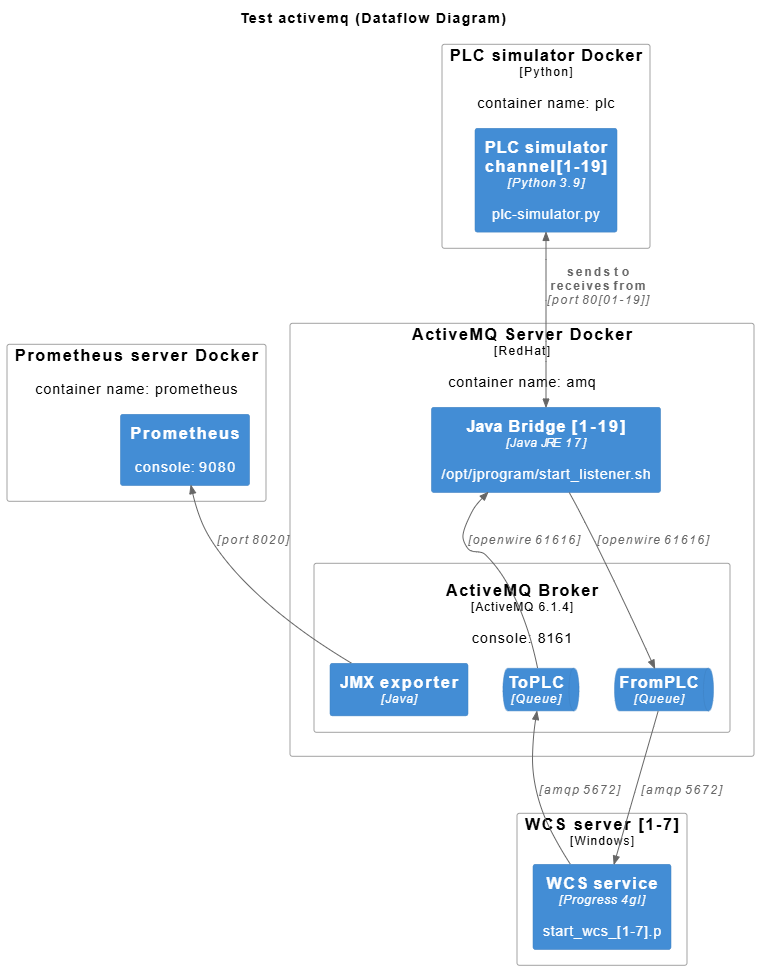
\includegraphics[width=.9\textwidth]{img/test_amq_dataflow.png}
  \caption{\label{fig:test_amq_dataflow}Dataflow test AMQ}
\end{figure}

\subsubsection{Installatie}
Het installeren van dit systeem is duidelijk uitgelegd in de officiële documentatie van Apache ActiveMQ.
Configuratie moet aangepast worden in ``activemq.xml'' om de service toegankelijk te maken voor externe services.
Daarnaast moet het bestand ``setenv'' aangepast worden om de metrics via ``jmx\_exporter'' beschikbaar te maken.

\subsubsection{Integratie}
Het WCS script kan de verbinding maken met de ActiveMQ server via poort 5672 door gebruik te maken van de JMS adapter.
De Java listeners gebruiken de JMS library en connecteren via het Openwire protocol op poort 16161.
Voor de monitoring wordt de ``jmx\_exporter'' gebruikt om de metrics beschikbaar te stellen voor externe software.
Hierdoor kan de monitoring data benaderd worden via een poort naar eigen keuze, in dit geval 8020.

\subsubsection{Performantie}
In deze test worden 19 PLC connecties gemaakt met de Java listeners die elk per 0.1 seconde een bericht versturen naar de  ``FromPLC'' queue.
Hierdoor worden meer dan 1680 berichten per minuut gesimuleerd en wordt er voldaan aan de minimale vereisten op gebied van performantie.
Het opmeten van deze test wordt verdeeld in twee categorieën, dequeued messages1680 en enqueued messages.
Om correct de throughput te meten moeten we beide categorieën meten omdat dit de volledige transactie representeert. 
\\\\
Volgende grafiek bevestigd dat er per minuut meer dan 1680 berichten kan geplaatst worden op de twee queues:
\begin{figure}[h!]
  \centering
  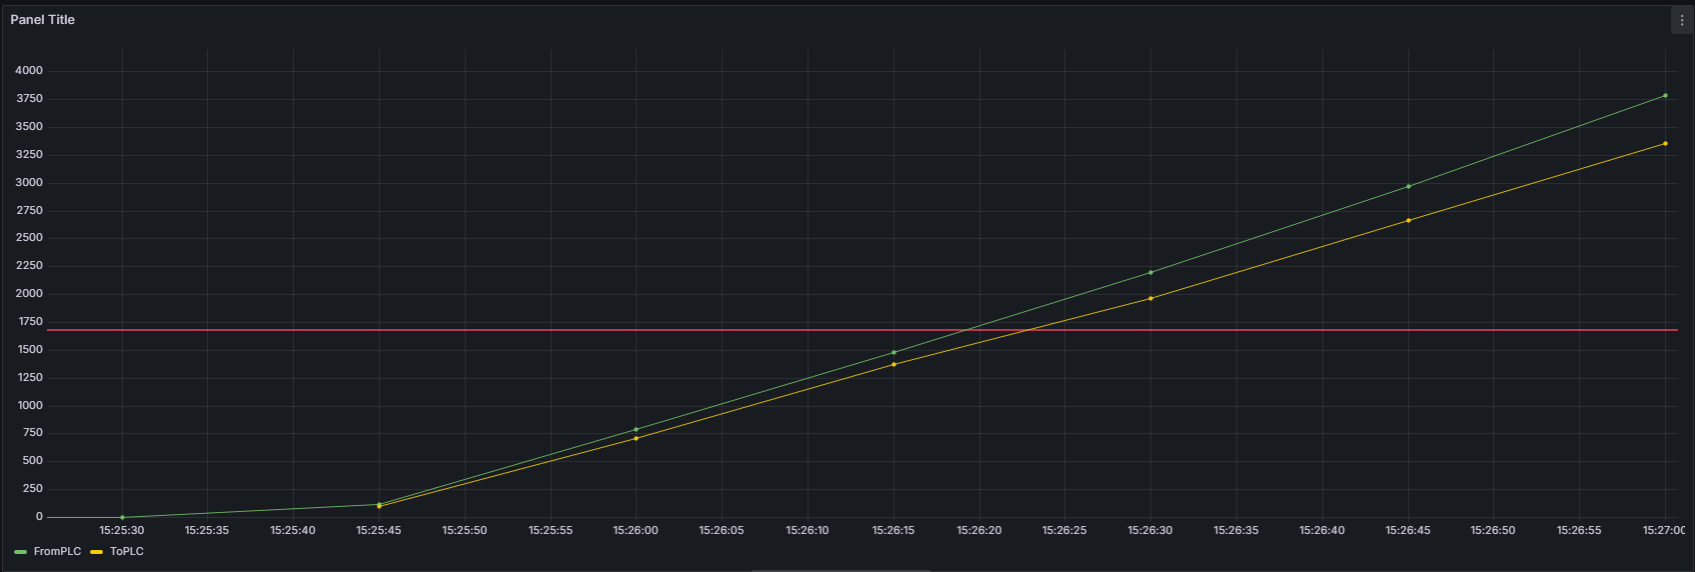
\includegraphics[width=.9\textwidth]{img/amq-enqueue-count.png}
  \caption{\label{fig:amq_enqueue_count}Enqueue ActiveMQ}
\end{figure}

Zoals de grafiek laat zien kan de message broker meer dan 1680 berichten naar de consumer versturen binnen de minuut.
\begin{figure}[h!]
  \centering
  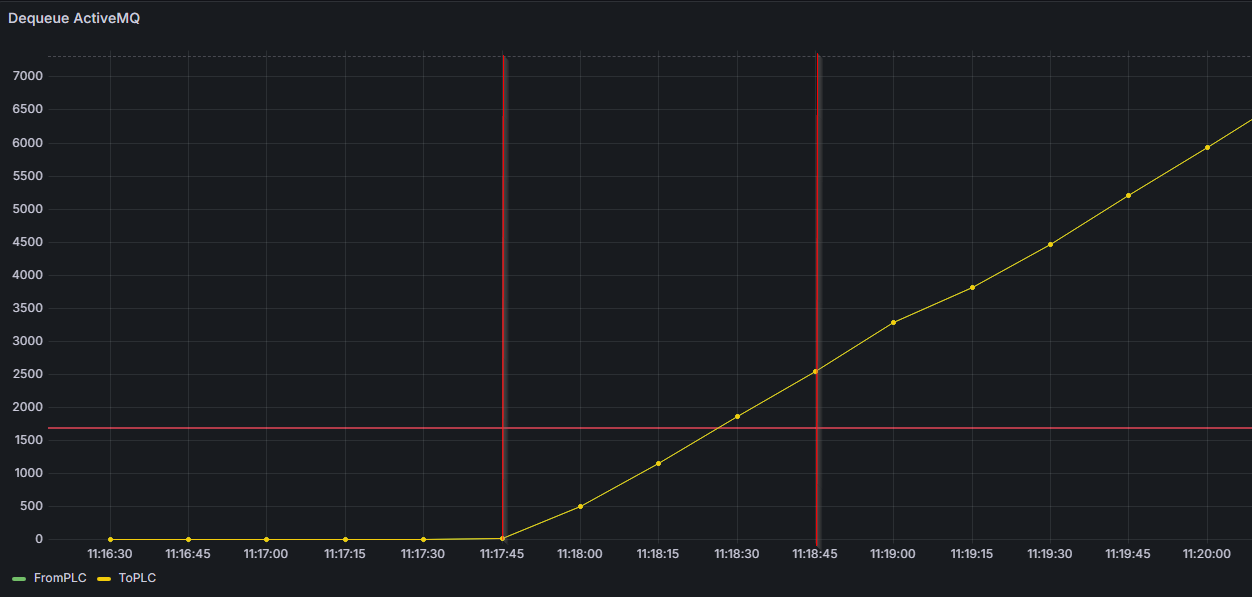
\includegraphics[width=.9\textwidth]{img/amq-dequeue-count.png}
  \caption{\label{fig:amq_dequeue_count}Dequeue ActiveMQ}
\end{figure}

\subsubsection{Samenvatting}
Installatie en integratie kon gebeuren zonder al te complexe aanpassingen.
Monitoring is mogelijk en gemakkelijk te verkrijgen. 
Er is ook een console beschikbaar waar de metrics kunnen geraadpleegd worden.
Qua performantie voldoet dit product en kan het over twee queues meer dan 1680 berichten verwerken.
  

\subsection{Test RabbitMQ}
\subsubsection{Installatie}
 
\subsubsection{Integratie}
 
Overzicht infrastructuur:
\begin{figure}[h!]
  \centering
  % \includegraphics[width=.5\textwidth]{img/test_rabbitmq_dataflow.png}
  \caption{\label{fig:test_rabbitmq_dataflow}Dataflow test RabbitMQ}
\end{figure}

\subsubsection{Performantie}
Volgende grafiek geeft weer hoeveel berichten er per minuut verzonden kunnen worden naar de message queue.


\subsection{Test Artemis}

\subsubsection{Installatie}
 
\subsubsection{Integratie}

Overzicht van de infrastructuur:
\begin{figure}[h!]
  \centering
  % \includegraphics[width=.5\textwidth]{img/test_artemis_dataflow.png}
  \caption{\label{fig:test_artemis_dataflow}Dataflow test Artemis}
\end{figure}

\subsubsection{Performantie}
Volgende grafiek geeft weer hoeveel berichten er per minuut verzonden kunnen worden naar de message queue.









